\documentclass[11pt,a4paper]{article}
\usepackage[utf8]{inputenc}
\usepackage[margin=1in]{geometry}
\usepackage{amsmath}
\usepackage{amsfonts}
\usepackage{amssymb}
\usepackage{tikz}
\usetikzlibrary{shapes.geometric, arrows, positioning}

% Define block styles for the flowchart with corrected text properties
\tikzset{
    startstop/.style={rectangle, rounded corners, minimum width=3cm, minimum height=1cm, text centered, draw=black, fill=red!20},
    process/.style={rectangle, minimum width=3cm, minimum height=1cm, text width=4cm, align=center, draw=black, fill=orange!20},
    decision/.style={diamond, minimum width=3cm, minimum height=1cm, text centered, draw=black, fill=blue!20, aspect=2},
    arrow/.style={thick,->,>=stealth}
}

\title{The Mathematical Logic of the 72 Melakarta Ragas}
\author{Carnatic Music Theory}
\date{}

\begin{document}

\maketitle

\section{Introduction}
The Melakarta system is a mathematical classification of the 72 parent scales in Carnatic music[cite: 4]. The logic is based on the permutation of the 12 swarasthanas within a heptatonic framework[cite: 4].

\section{The Logic Flowchart}

\begin{center}
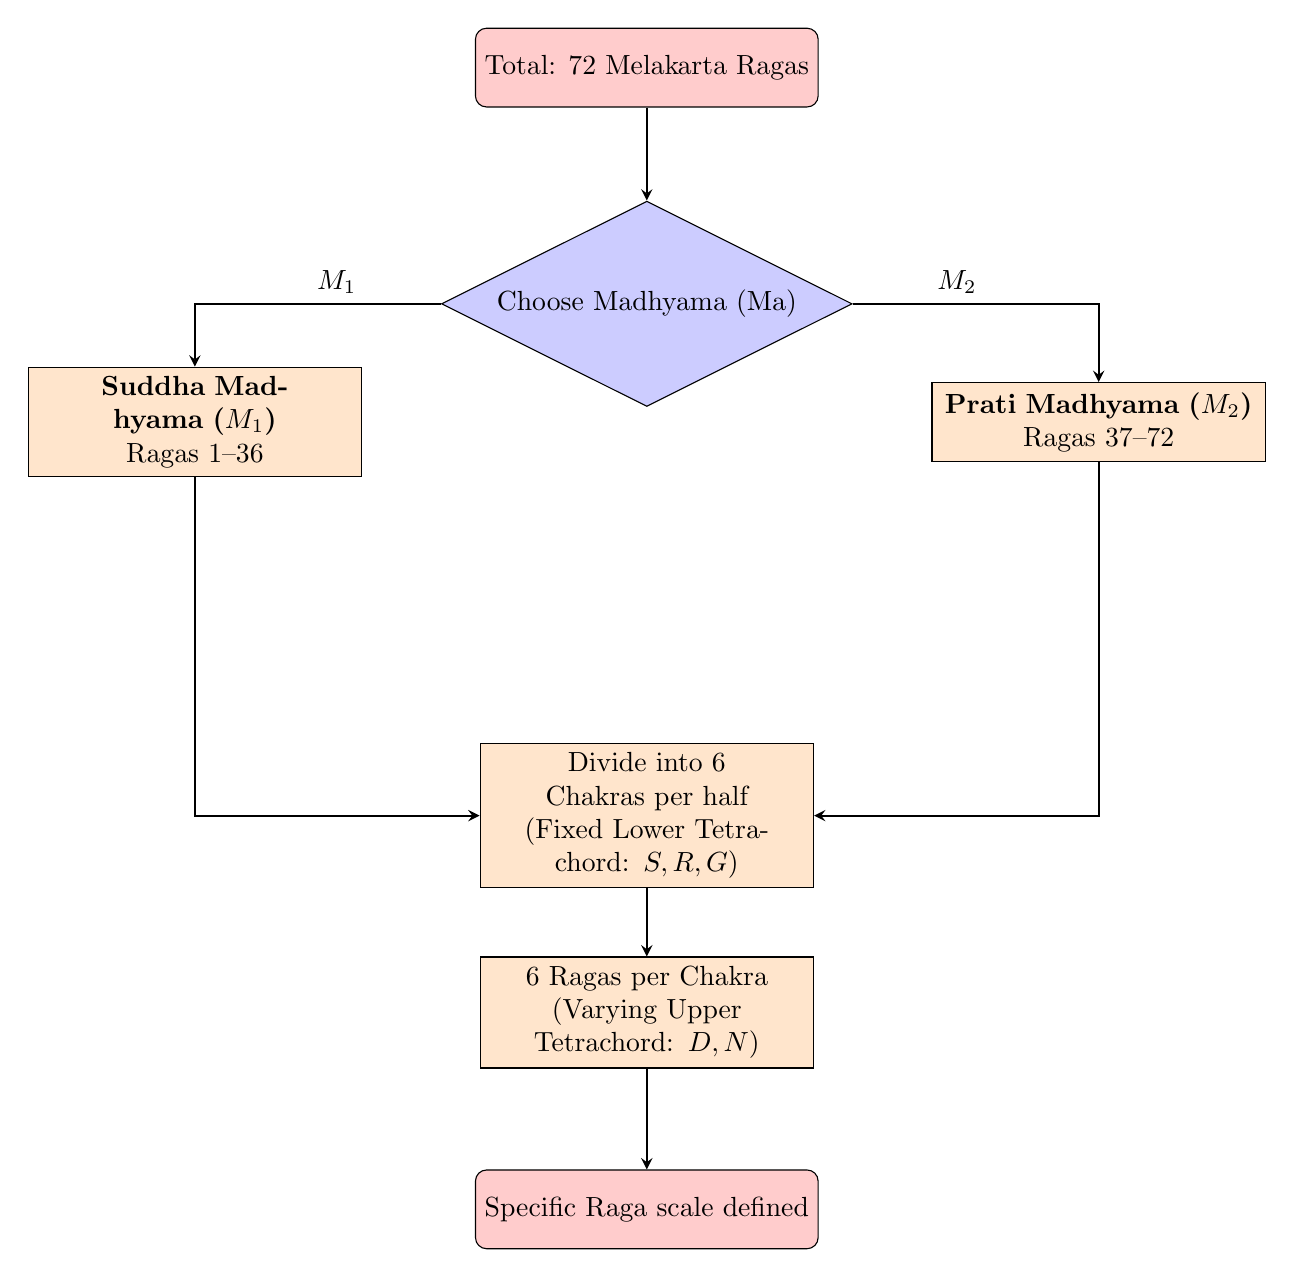
\begin{tikzpicture}[node distance=2.5cm, auto]

% Nodes
\node (start) [startstop] {Total: 72 Melakarta Ragas};
\node (dec1) [decision, below of=start, yshift=-0.5cm] {Choose Madhyama (Ma)};

\node (m1) [process, left=1cm of dec1, yshift=-1.5cm] {\textbf{Suddha Madhyama ($M_1$)} \\ Ragas 1--36};
\node (m2) [process, right=1cm of dec1, yshift=-1.5cm] {\textbf{Prati Madhyama ($M_2$)} \\ Ragas 37--72};

\node (chakra) [process, below of=dec1, yshift=-4cm] {Divide into 6 Chakras per half \\ (Fixed Lower Tetrachord: $S, R, G$)};
\node (raga) [process, below of=chakra] {6 Ragas per Chakra \\ (Varying Upper Tetrachord: $D, N$)};
\node (final) [startstop, below of=raga] {Specific Raga scale defined};

% Connectors
\draw [arrow] (start) -- (dec1);
\draw [arrow] (dec1) -| node[anchor=south, xshift=1.8cm] {$M_1$} (m1);
\draw [arrow] (dec1) -| node[anchor=south, xshift=-1.8cm] {$M_2$} (m2);
\draw [arrow] (m1) |- (chakra);
\draw [arrow] (m2) |- (chakra);
\draw [arrow] (chakra) -- (raga);
\draw [arrow] (raga) -- (final);

\end{tikzpicture}
\end{center}

\section{Structural Components}

\subsection{The Madhyama Split}
The division is based on the 4th note (Ma)[cite: 4]:
\begin{itemize}
    \item \textbf{Purva Melas (1--36):} Feature $M_1$[cite: 4].
    \item \textbf{Uttara Melas (37--72):} Feature $M_2$[cite: 4].
\end{itemize}

\subsection{The 12 Chakras (Purvanga)}
Within a Chakra, the notes $S, R, G$ are fixed[cite: 4]:
\begin{enumerate}
    \item \textbf{Indu:} $R_1, G_1$[cite: 4]
    \item \textbf{Netra:} $R_1, G_2$[cite: 4]
    \item \textbf{Agni:} $R_1, G_3$[cite: 4]
    \item \textbf{Veda:} $R_2, G_2$[cite: 4]
    \item \textbf{Bana:} $R_2, G_3$[cite: 4]
    \item \textbf{Rutu:} $R_3, G_3$[cite: 4]
\end{enumerate}

\subsection{The Internal Rotation (Uttaranga)}
The notes $P, D, N$ vary across the 6 ragas in each Chakra[cite: 4]:
\begin{enumerate}
    \item $D_1, N_1$[cite: 4]
    \item $D_1, N_2$[cite: 4]
    \item $D_1, N_3$[cite: 4]
    \item $D_2, N_2$[cite: 4]
    \item $D_2, N_3$[cite: 4]
    \item $D_3, N_3$[cite: 4]
\end{enumerate}

\section*{Key References}
\begin{itemize}
    \item Venkatamakhin, \textit{Chaturdandi Prakashika} (c. 1630)[cite: 4].
    \item Govindacharya, \textit{Sangraha Chudamani} (18th Century)[cite: 4].
    \item S. Bhagyalekshmy, \textit{Ragas in Carnatic Music}[cite: 4].
\end{itemize}

\end{document}
